\chapter{Lipids}\label{ch:b1:lipids}

A camel crossing a desert carries thirty kilograms of \omterm{def:b1:lipids:triglyceride}{fat} in its hump
and no water there at all; a trout in a mountain stream at
\qty{4}{\celsius} has membranes as fluid as a carp's in a warm pond;
and a drop of olive \omterm{def:b1:lipids:triglyceride}{oil} shaken into water breaks into a cloud of
droplets that, left alone, gather back into one. All three are \omterm{def:b1:lipids:fattyacid}{lipids}
at work: the densest store of chemical energy an \omterm{def:b1:organism-environment:organism}{organism} can carry,
the film that bounds every \omterm{def:b1:cell-unit-of-life:cell}{cell} and every \omterm{def:b1:cell-unit-of-life:prokeuk}{organelle}, and the class of
molecule that water refuses to dissolve. This chapter describes \omterm{def:b1:lipids:fattyacid}{fatty
acids} and the \omterm{def:b1:lipids:triglyceride}{fats} built from them, the \omterm{def:b1:lipids:amphiphilic}{amphiphilic} \omterm{def:b1:lipids:fattyacid}{lipids} that
assemble into membranes, what makes a membrane more or less fluid, and
the other \omterm{def:b1:lipids:fattyacid}{lipids} --- \omterm{def:b1:lipids:amphiphilic}{sterols}, pigments, hormones --- that a few carbons
arranged in rings and chains can be.

\section{Fatty acids}

\begin{definition}[Lipid, fatty acid]\label{def:b1:lipids:fattyacid}
\emph{Lipids}\index{lipid} are the biological molecules defined not by
a common structure but by a common property: they are insoluble in
water and soluble in non-polar solvents. Most are built on
\emph{fatty acids}\index{fatty acid}: carboxylic acids with an
unbranched hydrocarbon chain of \qtyrange{12}{24}{} carbons, almost
always an even number (they are assembled two carbons at a time,
\cref{ch:b1:biosyntheses-integration}). A \emph{saturated}\index{saturated fatty acid} fatty acid has only single bonds and a straight, flexible
chain; an \emph{unsaturated}\index{unsaturated fatty acid} one has one
or more double bonds, in the \emph{cis} configuration, each putting a
rigid kink of about $30^\circ$ in the chain. Notation: C18:1 $\Delta^9$
is an 18-carbon acid with one double bond after carbon 9 (oleic acid);
an \emph{omega-3} acid has its last double bond three carbons from the
methyl end.
\end{definition}

\begin{omfigure}
\begin{tikzpicture}[font=\footnotesize, line cap=round, line join=round]
  % stearic acid: zig-zag of 18 carbons
  \draw[very thick, omDef!80!black] (0,0) \foreach \i in {1,...,17} { -- ++({0.36}, {0.22*(-1)^\i}) };
  \node[fill=omThm!25, draw=omThm, rounded corners=2pt, inner sep=2pt] at (-0.1,0.0) {COOH};
  \node[anchor=east, align=right] at (-0.85,0) {stearic acid C18:0\\ saturated, straight\\ melts at \qty{70}{\celsius}};
  \node[anchor=west] at (6.3,-0.22) {$\mathrm{CH_3}$};
  % oleic acid: kink at carbon 9-10, second half tilted downward
  \draw[very thick, omDef!80!black] (0,-2.0) \foreach \i in {1,...,8} { -- ++({0.36}, {0.22*(-1)^\i}) };
  \draw[very thick, omDef!80!black] (2.88,-2.0) -- ++(0.36,0.22);
  \draw[double, very thick, omThm] (3.24,-1.78) -- ++(0.36,0.22);
  \draw[very thick, omDef!80!black] (3.60,-1.56) \foreach \i in {1,...,8} { -- ++({0.33}, {0.22*(-1)^(\i+1)-0.13}) };
  \node[fill=omThm!25, draw=omThm, rounded corners=2pt, inner sep=2pt] at (-0.1,-2.0) {COOH};
  \node[anchor=east, align=right] at (-0.85,-2.0) {oleic acid C18:1 $\Delta^9$\\ one \emph{cis} double bond, kinked\\ melts at \qty{13}{\celsius}};
  \node[omThm, anchor=south] at (3.42,-1.45) {\emph{cis} double bond};
  \node[anchor=west] at (6.35,-2.62) {$\mathrm{CH_3}$};
\end{tikzpicture}

{\small Two 18-carbon \omterm{def:b1:lipids:fattyacid}{fatty acids}. The saturated chain is straight and
packs closely against its neighbours; the \emph{cis} double bond of
oleic acid bends the chain and keeps neighbours apart, which is why
oleic acid is liquid at room temperature and stearic acid a solid.}
\end{omfigure}

\begin{proposition}[Melting points]\label{prop:b1:lipids:melting}
The melting point of a \omterm{def:b1:lipids:fattyacid}{fatty acid}, and the \omterm{def:b1:lipids:fluidity}{fluidity} of any \omterm{def:b1:lipids:fattyacid}{lipid}
assembly it belongs to, is set by how closely the chains can pack:
it rises with chain length (\qty{44}{\celsius} for C12:0,
\qty{63}{\celsius} for C16:0, \qty{70}{\celsius} for C18:0) and falls
sharply with each \emph{cis} double bond (C18:0 \qty{70}{\celsius},
C18:1 \qty{13}{\celsius}, C18:2 \qty{-5}{\celsius}, C18:3
\qty{-11}{\celsius}). Animal \omterm{def:b1:lipids:triglyceride}{fats}, rich in saturated acids, are solid
at room temperature; plant and fish \omterm{def:b1:lipids:triglyceride}{oils}, rich in unsaturated ones,
are liquid.
\end{proposition}
\begin{proof}
Straight chains lie side by side and every $\mathrm{CH_2}$ makes \omterm{def:b1:water-small-molecules:bonds}{van
der Waals} contacts with its neighbours, each worth a few kilojoules
per mole, summed along the chain: more carbons, more contacts, more
heat to separate them. A kink prevents close contact over several
carbons on each side and removes many contacts at once.
\end{proof}

\section{Fats: the energy store}

\begin{definition}[Triglyceride]\label{def:b1:lipids:triglyceride}
A \emph{triglyceride}\index{triglyceride} (triacylglycerol, a
\emph{fat}\index{fat} when solid, an \emph{oil}\index{oil} when liquid)
is glycerol --- a three-carbon alcohol --- esterified on its three
hydroxyls by three \omterm{def:b1:lipids:fattyacid}{fatty acids}. It has no charge and no polar group
left: it is entirely hydrophobic, and it is stored as anhydrous
droplets in \emph{adipocytes}\index{adipocyte}, \omterm{def:b1:cell-unit-of-life:cell}{cells} of the adipose
\omterm{def:b1:body-plans-tissues:tissue}{tissue} that are little more than a droplet of fat with a nucleus pushed
to one side.
\end{definition}

\begin{omfigure}
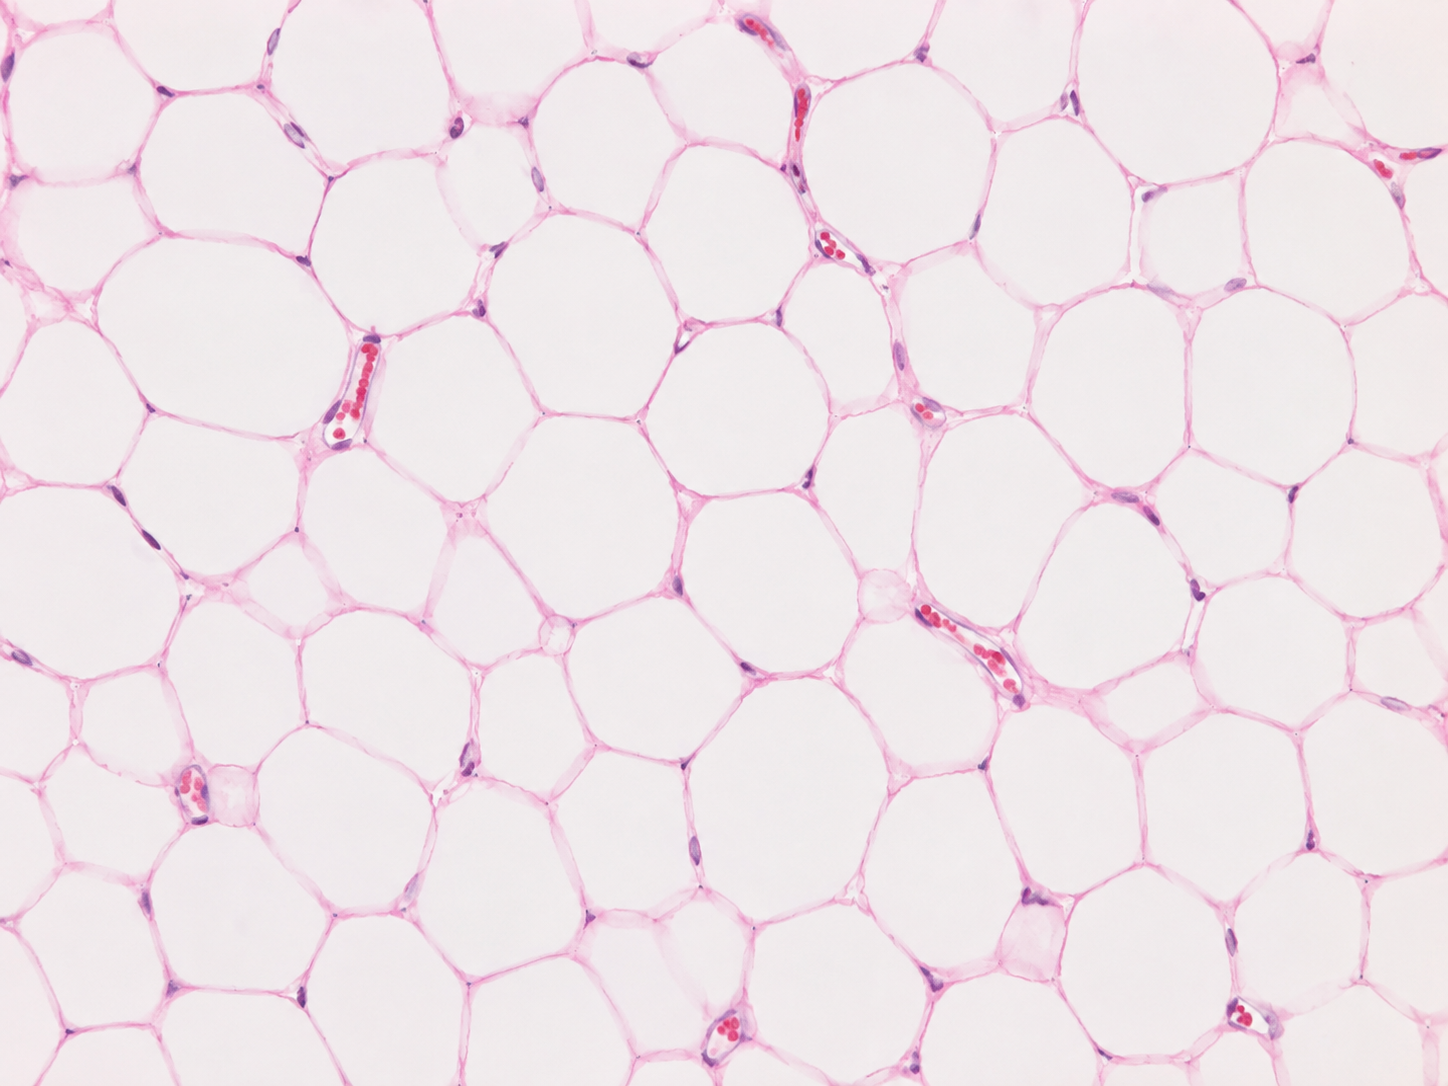
\includegraphics[width=0.5\linewidth]{images/book3/ai/b3-09-adipose-micrograph.png}

{\small White adipose \omterm{def:b1:body-plans-tissues:tissue}{tissue}: each \omterm{def:b1:cell-unit-of-life:cell}{cell} is one droplet of
\omterm{def:b1:lipids:triglyceride}{triglyceride}, up to \qty{100}{\micro m} across, with its \omterm{def:b1:cell-unit-of-life:cell}{cytoplasm} and
nucleus squeezed into a thin rim. Capillaries run between the \omterm{def:b1:cell-unit-of-life:cell}{cells} to
deliver and collect \omterm{def:b1:lipids:fattyacid}{fatty acids}.}
\end{omfigure}

\begin{proposition}[Fat is the densest energy store]\label{prop:b1:lipids:energystore}
Oxidising \qty{1}{g} of \omterm{def:b1:lipids:triglyceride}{fat} releases \qty{38}{kJ}, against \qty{17}{kJ}
for \qty{1}{g} of carbohydrate or protein: the carbons of a \omterm{def:b1:lipids:fattyacid}{fatty acid}
are more reduced (more C--H bonds, fewer C--O) and so give up more
electrons to oxygen. Moreover \omterm{def:b1:lipids:triglyceride}{fat} is stored dry, whereas glycogen binds
about \qty{3}{g} of water per gram: \qty{1}{g} of stored glycogen
yields \qty{4}{kJ} per gram of stored mass, \omterm{def:b1:lipids:triglyceride}{fat} nine times more. A lean
human carries \qty{0.5}{kg} of glycogen (a day's energy) and
\qty{12}{kg} of \omterm{def:b1:lipids:triglyceride}{fat} (more than a month's).
\end{proposition}

\begin{example}[Why not store everything as fat]\label{ex:b1:lipids:whyglycogen}
\omterm{def:b1:lipids:triglyceride}{Fat} can only be burnt with oxygen, slowly, and cannot be turned back
into glucose in animals (\cref{ch:b1:biosyntheses-integration}); the
brain and the red \omterm{def:b1:cell-unit-of-life:cell}{cells} need glucose, and a sprinting muscle needs it
faster than \omterm{def:b1:lipids:triglyceride}{fat} can supply. Glycogen is the fast, oxygen-free, glucose
store for hours; \omterm{def:b1:lipids:triglyceride}{fat}, the dense store for weeks. A migrating bird, a
hibernating dormouse and a camel are \omterm{def:b1:lipids:triglyceride}{fat}; a sprinter's legs are
glycogen.
\end{example}

\begin{definition}[Waxes]\label{def:b1:lipids:wax}
\emph{Waxes}\index{wax} are esters of a \omterm{def:b1:lipids:fattyacid}{fatty acid} with a long-chain
alcohol: solid, entirely hydrophobic, and used as coatings --- the
\omterm{def:b1:flowering-plant-organization:tissues}{cuticle} of \omterm{def:b1:flowering-plant-organization:organs}{leaves} (\cref{ch:b1:flowering-plant-organization}), the
surface of insects, the waterproofing of feathers and fur, the comb of
bees.
\end{definition}

\section{Membrane lipids and self-assembly}

\begin{definition}[Amphiphilic lipids]\label{def:b1:lipids:amphiphilic}
The \omterm{def:b1:lipids:fattyacid}{lipids} of membranes are \emph{amphiphilic}\index{amphiphilic molecule}: a polar \emph{head} that water solvates and one or two
non-polar \emph{tails} that it excludes.
\emph{Glycerophospholipids}\index{phospholipid} are glycerol bearing two
\omterm{def:b1:lipids:fattyacid}{fatty acids} and, on the third carbon, a phosphate linked to a small
polar alcohol (choline, ethanolamine, serine, inositol): phosphatidyl-choline
is the commonest \omterm{def:b1:lipids:fattyacid}{lipid} of animal membranes. \emph{Sphingolipids}\index{sphingolipid}
are built on the amino-alcohol sphingosine instead of glycerol, with
one \omterm{def:b1:lipids:fattyacid}{fatty acid} and a head of phosphocholine (sphingomyelin) or of
sugars (glycolipids), and are enriched in the outer leaflet and in
nerve sheaths. \emph{Sterols}\index{sterol} --- \emph{cholesterol}\index{cholesterol}
in animals, related sterols in plants and fungi --- are rigid four-ring
molecules with a single hydroxyl as their head, lying among the tails
of the other \omterm{def:b1:lipids:fattyacid}{lipids}.
\end{definition}

\begin{proposition}[Self-assembly]\label{prop:b1:lipids:selfassembly}
\index{self-assembly}\index{micelle}\index{liposome}
In water, \omterm{def:b1:lipids:amphiphilic}{amphiphilic molecules} assemble spontaneously so as to hide
their tails and expose their heads. The shape of the molecule decides
the structure: single-tailed \omterm{def:b1:lipids:fattyacid}{lipids} (\omterm{def:b1:lipids:fattyacid}{fatty acids}, detergents), shaped
like cones, form \emph{micelles} --- spheres a few nanometres across
with the tails inside; double-tailed \omterm{def:b1:lipids:amphiphilic}{phospholipids}, shaped like
cylinders, form \emph{bilayers}, which close on themselves into
\emph{liposomes} (vesicles) to leave no edge exposed. The assembly is
driven by the \omterm{prop:b1:water-small-molecules:properties}{hydrophobic effect} (\cref{ch:b1:water-small-molecules}):
it costs no energy and needs no enzyme, and a torn bilayer reseals by
itself. Membranes are self-healing sheets that grow by insertion of new
\omterm{def:b1:lipids:fattyacid}{lipids} and never form from nothing: every membrane comes from a
membrane.
\end{proposition}
\begin{proof}[Evidence]
Dried \omterm{def:b1:lipids:amphiphilic}{phospholipid} dispersed in water forms closed vesicles with
bilayer walls visible in the \omterm{prop:b1:cell-unit-of-life:microscopes}{electron microscope} (Bangham, 1965);
their permeability to ions and water matches that of \omterm{def:b1:cell-unit-of-life:cell}{cell} membranes,
and they can be loaded with drugs and fused with \omterm{def:b1:cell-unit-of-life:cell}{cells}. Adding a
detergent (single-tailed, cone-shaped) dissolves the bilayer into
mixed micelles; removing it by dialysis lets the bilayer reform.
\end{proof}

\begin{omfigure}
\begin{tikzpicture}[font=\footnotesize, line cap=round]
  % micelle: ring of heads with tails pointing inward
  \foreach \a in {0,30,...,330} {
    \fill[omDef!60] ({1.2*cos(\a)},{1.2*sin(\a)}) circle (0.14);
    \draw[omDef!70!black, thick] ({1.05*cos(\a)},{1.05*sin(\a)}) -- ({0.35*cos(\a)},{0.35*sin(\a)});
  }
  \node[anchor=north, align=center] at (0,-1.55) {micelle: single-tailed\\ lipids (cones)};
  % bilayer segment
  \foreach \i in {0,...,9} {
    \fill[omDef!60] (3.2+0.36*\i,0.75) circle (0.13); \draw[omDef!70!black, thick] (3.14+0.36*\i,0.62) -- (3.14+0.36*\i,0.1) (3.26+0.36*\i,0.62) -- (3.26+0.36*\i,0.1);
    \fill[omDef!60] (3.2+0.36*\i,-0.75) circle (0.13); \draw[omDef!70!black, thick] (3.14+0.36*\i,-0.62) -- (3.14+0.36*\i,-0.1) (3.26+0.36*\i,-0.62) -- (3.26+0.36*\i,-0.1);
  }
  \node[anchor=north, align=center] at (4.85,-1.55) {bilayer: double-tailed\\ lipids (cylinders)};
  % liposome: two concentric rings of heads with tails between
  \foreach \a in {0,15,...,345} {
    \fill[omDef!60] ({9.3+1.45*cos(\a)},{1.45*sin(\a)}) circle (0.11);
    \draw[omDef!70!black, thick] ({9.3+1.33*cos(\a)},{1.33*sin(\a)}) -- ({9.3+1.0*cos(\a)},{1.0*sin(\a)});
    \fill[omDef!60] ({9.3+0.62*cos(\a)},{0.62*sin(\a)}) circle (0.10);
    \draw[omDef!70!black, thick] ({9.3+0.72*cos(\a)},{0.72*sin(\a)}) -- ({9.3+0.98*cos(\a)},{0.98*sin(\a)});
  }
  \node at (9.3,0) {water};
  \node[anchor=north, align=center] at (9.3,-1.55) {liposome: a bilayer closed\\ on itself, no edges};
\end{tikzpicture}

{\small Three assemblies of \omterm{def:b1:lipids:amphiphilic}{amphiphilic} \omterm{def:b1:lipids:fattyacid}{lipids} in water. Cone-shaped
single-tailed molecules pack into micelles; cylindrical double-tailed
\omterm{def:b1:lipids:amphiphilic}{phospholipids} form a bilayer, which closes into a vesicle to hide its
edges.}
\end{omfigure}

\begin{omfigure}
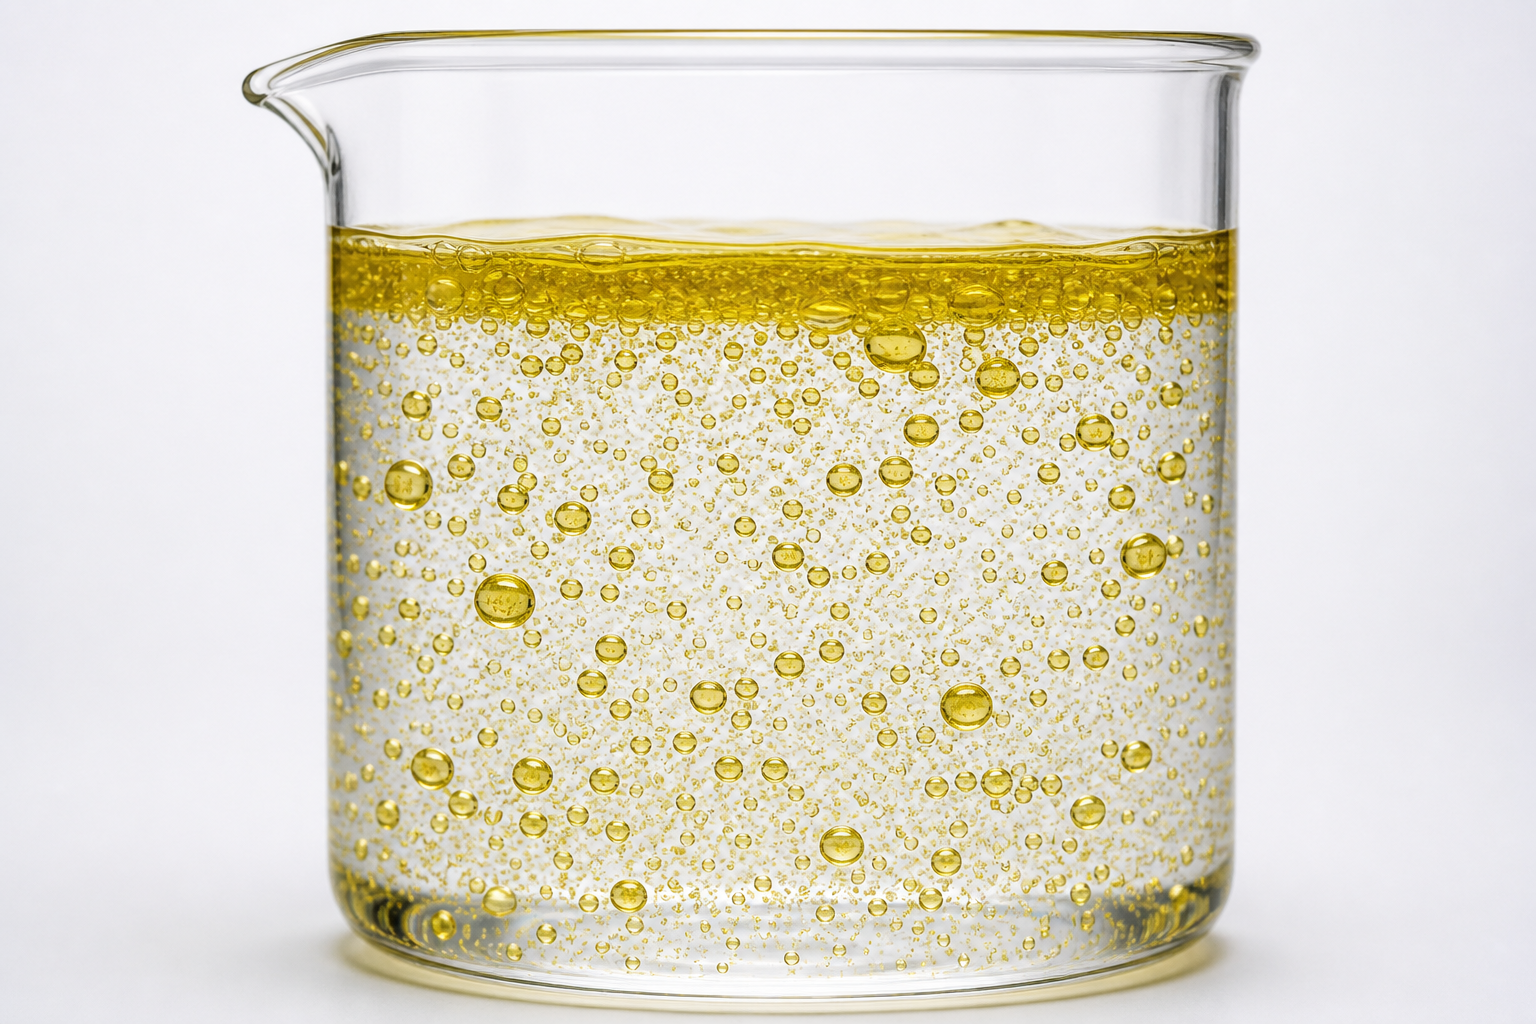
\includegraphics[width=0.5\linewidth]{images/book3/ai/b3-09-oil-water-emulsion.png}

{\small \omterm{def:b1:lipids:triglyceride}{Oil} shaken into water: a cloud of droplets that will coalesce
within minutes unless an amphiphile --- a detergent, a bile salt, a
\omterm{def:b1:lipids:amphiphilic}{phospholipid} --- coats them. Emulsification is what the gut does to
dietary \omterm{def:b1:lipids:triglyceride}{fat} before its enzymes can reach it.}
\end{omfigure}

\begin{example}[Bile salts]\label{ex:b1:lipids:bile}
Dietary \omterm{def:b1:lipids:triglyceride}{fat} arrives in the intestine as \omterm{def:b1:lipids:triglyceride}{oil}; the lipase that digests it
works only at the oil--water interface. Bile salts, \omterm{def:b1:lipids:amphiphilic}{amphiphilic}
derivatives of \omterm{def:b1:lipids:amphiphilic}{cholesterol}, coat the \omterm{def:b1:lipids:triglyceride}{fat} into droplets a micrometre
across, multiplying the interface a thousandfold, and then carry the
\omterm{def:b1:lipids:fattyacid}{fatty acids} released, in micelles, to the absorbing \omterm{def:b1:cell-unit-of-life:cell}{cells}
(\cref{ch:b1:digestion-absorption}). The same trick is used by soap.
\end{example}

\section{Membrane fluidity}

\begin{definition}[Fluidity, phase transition]\label{def:b1:lipids:fluidity}
A \omterm{def:b1:membranes-transport:membrane}{lipid bilayer} has a \emph{phase transition temperature}\index{phase transition temperature} $T_m$: below it the chains are packed in an
ordered, gel-like state in which \omterm{def:b1:lipids:fattyacid}{lipids} barely move; above it they are
disordered and the bilayer is a two-dimensional fluid in which a \omterm{def:b1:lipids:fattyacid}{lipid}
changes places with its neighbour a million times a second and crosses
the membrane's plane at \qty{1}{\micro m/s}. \omterm{def:b1:cell-unit-of-life:cell}{Cells} keep their membranes
above $T_m$: the \emph{fluidity}\index{membrane fluidity} lets proteins
diffuse and rotate, vesicles bud and fuse, and the bilayer reseal.
\end{definition}

\begin{proposition}[What sets the fluidity]\label{prop:b1:lipids:fluidityfactors}
$T_m$ rises with the length of the chains and falls with their
unsaturation, as for free \omterm{def:b1:lipids:fattyacid}{fatty acids}; a bilayer of C18:0 chains melts
at \qty{55}{\celsius}, one of C18:1 chains at \qty{-20}{\celsius}.
\omterm{def:b1:lipids:amphiphilic}{Cholesterol}, inserted among the tails, has a double effect: above
$T_m$ its rigid rings restrict the motion of the chains and stiffen
the membrane; below $T_m$ they prevent the chains from packing and keep
it from freezing. It broadens the transition into a gradual change and
keeps the \omterm{def:b1:lipids:fluidity}{fluidity} nearly constant over a wide range of temperature ---
a \omterm{def:b1:water-small-molecules:buffer}{buffer} of \omterm{def:b1:lipids:fluidity}{fluidity}. Animal plasma membranes are up to one \omterm{def:b1:lipids:amphiphilic}{cholesterol}
for every \omterm{def:b1:lipids:amphiphilic}{phospholipid}.
\end{proposition}

\begin{omfigure}
\begin{tikzpicture}
\begin{axis}[
  width=0.86\linewidth, height=6.0cm,
  axis x line=bottom, axis y line=left,
  xmin=-20, xmax=60, ymin=0, ymax=1.15,
  xlabel={temperature (\unit{\celsius})}, ylabel={fluidity (relative)},
  xlabel style={font=\small, at={(axis description cs:0.5,-0.12)}, anchor=north},
  ylabel style={font=\small},
  tick label style={font=\small}, xtick={-20,0,20,40,60}, ytick={0,0.5,1},
  legend style={font=\small, at={(0.03,0.97)}, anchor=north west, draw=none},
  clip=false,
]
\addplot[very thick, omDef, domain=-20:60, samples=120] {1/(1+exp(-(x-41)/1.5))};
\addlegendentry{saturated C16 chains, no cholesterol}
\addplot[very thick, omProp, domain=-20:60, samples=120] {1/(1+exp(-(x+5)/1.5))};
\addlegendentry{one \emph{cis} double bond per lipid}
\addplot[very thick, omThm, domain=-20:60, samples=120] {0.15+0.7/(1+exp(-(x-20)/12))};
\addlegendentry{saturated chains with \qty{30}{\%} cholesterol}
\draw[dashed, gray] (axis cs:37,0) -- (axis cs:37,1.05);
\node[font=\scriptsize, anchor=south] at (axis cs:37,1.06) {\qty{37}{\celsius}};
\end{axis}
\end{tikzpicture}

{\small \omterm{def:b1:lipids:fluidity}{Fluidity} against temperature for three bilayers. Saturated
chains freeze sharply near \qty{40}{\celsius}; one double bond per
\omterm{def:b1:lipids:fattyacid}{lipid} lowers the transition below zero; \omterm{def:b1:lipids:amphiphilic}{cholesterol} smooths the
transition into a gentle slope, keeping the membrane neither solid nor
too fluid across the physiological range.}
\end{omfigure}

\begin{proposition}[Homeoviscous adaptation]\label{prop:b1:lipids:homeoviscous}
\index{homeoviscous adaptation}
\omterm{def:b1:organism-environment:organism}{Organisms} that cannot regulate their temperature adjust the composition
of their membranes to keep the \omterm{def:b1:lipids:fluidity}{fluidity} constant: as the temperature
falls, they replace saturated by \omterm{def:b1:lipids:fattyacid}{unsaturated fatty acids} and long
chains by shorter ones, and the reverse when it rises.
\end{proposition}
\begin{proof}[Evidence]
\emph{E. coli} grown at \qty{10}{\celsius} has twice the proportion of
\omterm{def:b1:lipids:fattyacid}{unsaturated fatty acids} of the same strain grown at \qty{40}{\celsius},
and the membranes of the two cultures, measured by the mobility of a
probe, are equally fluid at their growth temperatures. Trout
acclimated to \qty{5}{\celsius} carry more polyunsaturated acids in
their membrane \omterm{def:b1:lipids:fattyacid}{lipids} than trout at \qty{20}{\celsius}; the \omterm{def:b1:lipids:triglyceride}{fat} of
reindeer legs, close to the snow, is more unsaturated than the \omterm{def:b1:lipids:triglyceride}{fat} of
the trunk. Plants that survive frost enrich their membranes in
unsaturated \omterm{def:b1:lipids:fattyacid}{lipids} in autumn, and mutants unable to do so die when
chilled.
\end{proof}

\begin{example}[Butter, olive oil, fish oil]\label{ex:b1:lipids:kitchen}
Butter (\qty{65}{\%} saturated) is solid in the refrigerator and soft
at room temperature; olive \omterm{def:b1:lipids:triglyceride}{oil} (\qty{75}{\%} oleic acid) is liquid at
room temperature and clouds in the refrigerator; fish \omterm{def:b1:lipids:triglyceride}{oil}, rich in
omega-3 acids with five and six double bonds, stays liquid at
\qty{-20}{\celsius}, which is what a cod's membranes need in the North
Atlantic.
\end{example}

\section{Sterols, pigments and signals}

\begin{definition}[Steroids, isoprenoids]\label{def:b1:lipids:steroids}
\emph{Steroids}\index{steroid} share \omterm{def:b1:lipids:amphiphilic}{cholesterol}'s four fused rings:
\omterm{def:b1:lipids:amphiphilic}{cholesterol} itself (membranes, and the precursor of the rest), the bile
salts, vitamin D, and the steroid hormones --- cortisol, aldosterone,
the sex hormones --- small, hydrophobic molecules that cross membranes
freely and act on receptors inside the \omterm{def:b1:cell-unit-of-life:cell}{cell}. \emph{Isoprenoids}\index{isoprenoid}
(terpenes) are chains and rings of five-carbon isoprene units: the
\emph{carotenoids} that colour carrots and protect \omterm{def:b1:eukaryotic-cell:plastid}{chloroplasts}
(\cref{ch:b1:photosynthesis}), the side chain of chlorophyll, the
quinones of the electron-transport chains, rubber, and the fat-soluble
vitamins A, E and K.
\end{definition}

\begin{proposition}[What lipids do]\label{prop:b1:lipids:functions}
Energy storage (\omterm{def:b1:lipids:triglyceride}{triglycerides}); membranes (\omterm{def:b1:lipids:amphiphilic}{phospholipids}, \omterm{def:b1:lipids:amphiphilic}{sphingolipids},
\omterm{def:b1:lipids:amphiphilic}{sterols}); insulation and waterproofing (\omterm{def:b1:lipids:triglyceride}{fat}, \omterm{def:b1:lipids:wax}{waxes}); light absorption
and protection (carotenoids); electron carriage (quinones); signalling
between \omterm{def:b1:cell-unit-of-life:cell}{cells} (\omterm{def:b1:lipids:steroids}{steroid} hormones, prostaglandins) and within them
(inositol \omterm{def:b1:lipids:amphiphilic}{phospholipids}, diacylglycerol); vitamins. One property ---
insolubility in water --- underlies all of them: a \omterm{def:b1:lipids:fattyacid}{lipid} stays where it
is put, in a droplet, a film or a membrane, or crosses a membrane
without a carrier.
\end{proposition}

\begin{example}[A hormone that needs no receptor at the surface]\label{ex:b1:lipids:steroidhormone}
Cortisol, secreted by the adrenal gland, travels in the blood bound to a
carrier protein, \omterm{def:b1:flowering-plant-organization:organs}{leaves} it at a target \omterm{def:b1:cell-unit-of-life:cell}{cell}, dissolves through the
plasma membrane in seconds, and binds a receptor in the \omterm{def:b1:eukaryotic-cell:organelle}{cytosol} that
then enters the nucleus and switches genes on
(\cref{ch:b1:expression-control}). A protein hormone such as insulin,
water-soluble and too large to cross, must bind a receptor on the
outside and have its message relayed inward. The chemistry of the
messenger decides the route of the message.
\end{example}

\section{Exercises}

\begin{exercise}[$\star$]\label{exo:b1:lipids:1}
Define a \omterm{def:b1:lipids:fattyacid}{lipid} and explain why the definition is by property rather
than by structure.
\end{exercise}

\begin{exercise}[$\star$]\label{exo:b1:lipids:2}
Write the notation of linoleic acid (18 carbons, double bonds after
carbons 9 and 12) and say whether it is an omega-3 or an omega-6 acid.
\end{exercise}

\begin{exercise}[$\star$]\label{exo:b1:lipids:3}
Why does a \omterm{def:b1:lipids:triglyceride}{triglyceride} form droplets while a \omterm{def:b1:lipids:amphiphilic}{phospholipid} forms
bilayers? What structural difference is responsible?
\end{exercise}

\begin{exercise}[$\star$]\label{exo:b1:lipids:4}
From the \omterm{def:b1:lipids:fluidity}{fluidity} figure, at what temperature is each of the three
bilayers half-way through its transition? Which would you expect in a
bacterium living at \qty{10}{\celsius}?
\end{exercise}

\begin{exercise}[$\star\star$]\label{exo:b1:lipids:5}
A person stores \qty{15}{kg} of \omterm{def:b1:lipids:triglyceride}{fat}. Compute the energy it holds, the
number of days it could sustain a resting expenditure of
\qty{8}{MJ/d}, and the mass of hydrated glycogen that would hold the
same energy.
\end{exercise}

\begin{exercise}[$\star\star$]\label{exo:b1:lipids:6}
Rank by melting point: C14:0, C18:0, C18:1, C18:3, C22:0, and justify
each step of the ranking.
\end{exercise}

\begin{exercise}[$\star\star$]\label{exo:b1:lipids:7}
A red blood \omterm{def:b1:cell-unit-of-life:cell}{cell} has a surface of \qty{140}{\micro m^2}; a \omterm{def:b1:lipids:amphiphilic}{phospholipid}
head occupies \qty{0.6}{nm^2}. Compute the number of \omterm{def:b1:lipids:amphiphilic}{phospholipid}
molecules in the membrane (two leaflets) and, at \qty{750}{g/mol},
their total mass in picograms.
\end{exercise}

\begin{exercise}[$\star\star$]\label{exo:b1:lipids:8}
\qty{1}{g} of olive \omterm{def:b1:lipids:triglyceride}{oil} (density \qty{0.9}{g/mL}) is emulsified into
droplets of \qty{1}{\micro m} diameter. Compute the total interface
area. Repeat for a single drop. Why does the pancreatic lipase need the
emulsion?
\end{exercise}

\begin{exercise}[$\star\star$]\label{exo:b1:lipids:9}
Explain the two opposite effects of \omterm{def:b1:lipids:amphiphilic}{cholesterol} on \omterm{def:b1:lipids:fluidity}{membrane fluidity}
and why a membrane with \omterm{def:b1:lipids:amphiphilic}{cholesterol} has no sharp transition.
\end{exercise}

\begin{exercise}[$\star\star\star$]\label{exo:b1:lipids:10}
A mutant plant cannot make \omterm{def:b1:lipids:fattyacid}{unsaturated fatty acids}. Predict its
membranes at \qty{25}{\celsius} and at \qty{5}{\celsius}, what happens
to its \omterm{def:b1:cell-unit-of-life:cell}{cells} on a cold night, and why the wild type survives.
\end{exercise}

\begin{exercise}[$\star\star\star$]\label{exo:b1:lipids:11}
\omterm{def:b1:lipids:triglyceride}{Fat} gives \qty{1.07}{g} of water per gram oxidised (glycogen
\qty{0.56}{g}, protein \qty{0.4}{g}). Compute the water produced by a
camel oxidising \qty{1}{kg} of \omterm{def:b1:lipids:triglyceride}{fat}. The oxygen needed is
\qty{2}{L} per gram of \omterm{def:b1:lipids:triglyceride}{fat}; breathing it in dry desert air costs about
\qty{0.03}{g} of water per litre of air ventilated, at \qty{5}{\%}
oxygen extraction. Compute the water lost in breathing and say whether
the hump is a water store.
\end{exercise}

\begin{exercise}[$\star\star\star$]\label{exo:b1:lipids:12}
``A membrane assembles itself, but a \omterm{def:b1:cell-unit-of-life:cell}{cell} cannot make a membrane from
nothing.'' Reconcile the two halves of the sentence in a paragraph,
using the \omterm{prop:b1:water-small-molecules:properties}{hydrophobic effect}, the growth of membranes by insertion, and
the continuity of membranes through \omterm{def:b1:cell-unit-of-life:cell}{cell} division.
\end{exercise}

\section{Problem: Cold Water and Desert Fat}

\begin{problem}[{Weekend problem --- a trout's membranes in a mountain
stream and a camel's hump in the desert: unsaturation, transition
temperatures, energy density and metabolic water, ending on the mass
that storing fat instead of glycogen saves}]
\label{pb:b1:lipids:1}
Part I concerns a trout whose membrane \omterm{def:b1:lipids:amphiphilic}{phospholipids} carry chains of
C16:0, C18:1 and C22:6 (an omega-3 acid with six double bonds). Part II
concerns a dromedary of \qty{500}{kg} with a \qty{30}{kg} hump of
\omterm{def:b1:lipids:triglyceride}{triglyceride}, crossing a desert at a \omterm{def:b1:organism-environment:allometry}{metabolic rate} of
\qty{60}{MJ/d}. Energy: \omterm{def:b1:lipids:triglyceride}{fat} \qty{38}{kJ/g}, glycogen \qty{17}{kJ/g}
dry, stored with \qty{3}{g} of water per gram. Metabolic water:
\qty{1.07}{g/g} of \omterm{def:b1:lipids:triglyceride}{fat}. Oxygen: \qty{2.0}{L} per gram of \omterm{def:b1:lipids:triglyceride}{fat}; air is
\qty{21}{\%} oxygen; the camel extracts \qty{5}{\%} of the oxygen it
breathes; exhaled air carries \qty{30}{g/m^3} of water more than the
desert air inhaled.

\medskip
\noindent\textbf{Part I --- The trout.}
Trout acclimated to \qty{20}{\celsius} have membrane chains that are
\qty{40}{\%} C16:0, \qty{45}{\%} C18:1 and \qty{15}{\%} C22:6; trout at
\qty{5}{\celsius}, \qty{25}{\%}, \qty{40}{\%} and \qty{35}{\%}.
\begin{enumerate}
  \item Write the notation of the three acids and count the double
        bonds per chain in each.
  \item Compute the mean number of double bonds per chain at each
        temperature.
  \item Explain, from chain packing, why the change lowers the
        transition temperature of the membrane.
  \item A bilayer's $T_m$ falls by about \qty{20}{\celsius} for each
        additional \qty{0.5}{} double bond per chain on average. Estimate
        the shift of $T_m$ between the two trout.
  \item The warm trout's membrane is fluid at \qty{20}{\celsius} but
        would gel at \qty{5}{\celsius}. What would happen to its
        transport proteins, its pumps and its nerve conduction on a
        sudden cold night?
  \item The adaptation takes days. Name the enzymes the trout must
        make more of, and where in the \omterm{def:b1:cell-unit-of-life:cell}{cell} they act (\cref{ch:b1:eukaryotic-cell}).
  \item \omterm{def:b1:lipids:amphiphilic}{Cholesterol} is at one molecule per two \omterm{def:b1:lipids:amphiphilic}{phospholipids} in both
        trout. Explain what it contributes in each case.
\end{enumerate}

\medskip
\noindent\textbf{Part II --- The camel's energy.}
\begin{enumerate}[resume]
  \item Compute the energy stored in the hump.
  \item For how many days of the crossing does it suffice?
  \item Compute the mass of dry glycogen holding the same energy, and
        the mass of hydrated glycogen.
  \item Compute the mass saved by storing \omterm{def:b1:lipids:triglyceride}{fat} rather than glycogen, and
        express it as a fraction of the camel's body mass.
  \item \omterm{def:b1:lipids:triglyceride}{Fat} is stored in a hump rather than spread under the skin.
        Propose a reason, from the \omterm{prop:b1:mammal-organization:heatbudget}{heat budget} of
        \cref{ch:b1:mammal-organization}.
\end{enumerate}

\medskip
\noindent\textbf{Part III --- Is the hump a water store?}
\begin{enumerate}[resume]
  \item Compute the metabolic water produced by oxidising the whole
        hump.
  \item Compute the oxygen needed, in litres.
  \item Compute the volume of air the camel must ventilate to obtain
        it.
  \item Compute the water lost in exhaling that air.
  \item Compare the water gained with the water lost, and conclude.
  \item Instead of sweating, the camel lets its body temperature rise
        by \qty{6}{\celsius} during the day and cool at night. Compute
        the heat it stores this way (heat capacity
        \qty{3.5}{kJ.kg^{-1}.K^{-1}}) and the water that evaporating
        the same heat would cost (\qty{2.4}{kJ/g}).
  \item A camel can lose \qty{25}{\%} of its body water and survive,
        and its red \omterm{def:b1:cell-unit-of-life:cell}{cells} swell to twice their volume without bursting
        when it drinks \qty{100}{L} in ten minutes. Relate the second
        property to the membranes of \cref{ch:b1:membranes-transport}.
\end{enumerate}

\medskip
\noindent\textbf{Part IV --- The bilayer's arithmetic.}
A \omterm{def:b1:lipids:amphiphilic}{phospholipid} head occupies \qty{0.65}{nm^2}; a bilayer is
\qty{5}{nm} thick; the camel's red \omterm{def:b1:cell-unit-of-life:cell}{cells} have a surface of
\qty{80}{\micro m^2} and number $\num{8e12}$ per litre of blood.
\begin{enumerate}[resume]
  \item Compute the number of \omterm{def:b1:lipids:amphiphilic}{phospholipids} in one \omterm{def:b1:cell-unit-of-life:cell}{red-cell} membrane.
  \item Compute the number in all the red \omterm{def:b1:cell-unit-of-life:cell}{cells} of \qty{40}{L} of blood.
  \item At \qty{750}{g/mol}, compute the mass of that \omterm{def:b1:lipids:fattyacid}{lipid} in grams.
  \item A \omterm{def:b1:lipids:amphiphilic}{phospholipid} flips from one leaflet to the other
        spontaneously about once a week, but diffuses laterally
        \qty{1}{\micro m} in a second. Explain both numbers from the
        \omterm{prop:b1:water-small-molecules:properties}{hydrophobic effect}.
  \item Explain why, given the flip rate, the two leaflets of a
        membrane can stay different in composition for the life of a
        \omterm{def:b1:cell-unit-of-life:cell}{cell}.
  \item State the result: the mass the camel saves by carrying
        \qty{30}{kg} of \omterm{def:b1:lipids:triglyceride}{fat} rather than the glycogen of equal energy,
        and the verdict on the hump as a water store.
\end{enumerate}
\end{problem}
